\section{Modellierung}
\label{sec:modellierung}

\subsection{Ansatz über die Übertragsfunktion}
\label{sec:ansatzfunktion}

Der erste untersuchte Ansatz war das Modell in zwei getrennte System zu zerlegen und getrennt zu betrachten.
Die Annahme war, dass der Isolator lediglich als Filter auf das Antwortspektrum wirkt.

\begin{figure}[H]
    \centering
    \includegraphics[width=0.7\textwidth]{composition.png}
    \caption{Komposition}
    \label{fig:composition}
\end{figure}

Die Funktion $H(\omega)$ stellt hier das Antwortspektrum dar und $G(s)$ die Übertragungsfunktion des Isolators.
Sie kann mittels der Laplace-Transformation

\begin{equation} \label{laplace}
F(s) = \int_{0}^{\infty} f(t)e^{-st}dt
\end{equation}

aus der Bewegungsgleichung des Isolators \cite{Kramer}

\begin{equation}\label{eq:bewegungsgleichung}
c_i \cdot \dot x(t) + k_i \cdot x(t) = - m_i \cdot \ddot x(t)
\end{equation}

für eine Kraftanregung zu

\begin{equation} \label{laplace2}
G(s)=\frac{X(s)}{F(s)} = \frac{1}{m_i \cdot s^2 + c_i \cdot s + k_i}
\end{equation}

bestimmt (wobei $s = i \omega$) und das isolierte Antwortspektrum ($H(\omega) \cdot |G(s)|$) gewonnen werden da der Betrag der Übertragungsfunktion den Amplitudengang angibt.

Allerdings war dieser Ansatz nicht zielführend, da (wie an den Bewegungsdifferetialgleichungen (\cref{eq:BewegDGL}) erkennbar ist) die Systeme gekoppelt sind und nicht getrennt betrachtet werden können.

\subsection{Vereinfachter Ansatz}
\label{sec:ansatzvereinfacht}

\subsection{Ansatz über die Transmissibilität}
\label{sec:ansatztrasnm}

\subsubsection{Transmissibilität}
\label{sec:transm}



\begin{figure}[ht]
    \centering
    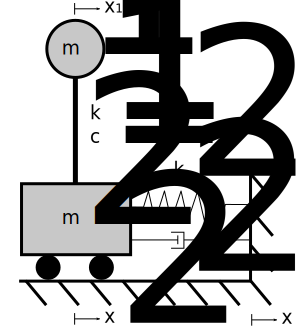
\includegraphics[width=0.5\textwidth]{voigt-kelvin-model.png}
    \caption{Voigt-Kelvin-Modell}
\end{figure}

\begin{align}\label{eq:BewegDGL}
\ddot x_1 m_1 &= -(x_1 - x_2) k_1 -(\dot x_1 - \dot x_2) c_1\\
\ddot x_2 m_2 &= (x_1 - x_2) k_1 + (\dot x_1 - \dot x_2) c_1 - (x_2 - x_3) k_2 - (\dot x_2 - \dot x_3) c_2
\end{align}

Ansatz für harmonische Schwingung:

\begin{align*}
x_j &= S_j e^{i \omega t}\\
\dot x_j &= i \omega S_j e^{i \omega t}\\
\ddot x_j &= - \omega^2 S_j e^{i \omega t}
\end{align*}

\begin{align}
- \omega^2 S_1 m_1 e^{i \omega t} &= - (S_1 - S_2) e^{i \omega t} k_1 - (S_1 - S_2) i \omega c_1 e^{i \omega t} \label{eq:2DOF1} \\
- \omega^2 S_2 m_2 e^{i \omega t} &= (S_1 - S_2)(k_1 + i \omega c_1) e^{i \omega t} - (S_2 - S_3)(k_2 + i \omega c_2) e^{i \omega t} \label{eq:2DOF2}
\end{align}

\cref{eq:2DOF1} nach $S_2$ umgestellt:

\begin{align*}
\omega^2 S_1 m_1 &= (S_1 - S_2)(k_1 + i \omega c_1) \\
&\Rightarrow X_1 = \frac{\omega^2 m_1}{k_1 + i \omega c_1}\\
S_2 &= S_1 (1 - X_1)
\intertext{$S_2$ in \cref{eq:2DOF2} eingesetzt:}
\omega^2 m_2 S_1 &= - (S_1 - S_1 (1 - X_1)) (k_1 + i \omega c_1) + (S_1 (1 - X_1) - S_3) (k_2 + i \omega c_2)\\
&\Rightarrow X_2 = \frac{\omega^2 m_2}{k_2 + i \omega c_2}\\
S_1 (1 - X_1) X_2 &= S_1 (1-X_1) - S_3 - S_1 X_1 \frac{k_1 + i \omega c_1}{k_2 + i \omega c_2}\\
&\Rightarrow X_{12} = \frac{\omega^2 m_1}{k_2 + i \omega c_2}\\
S_1 (1 - X_1)(X_2 - 1) &= S_3 + S_1 X_{12}\\
S_3 &= S_1 [(1 - X_1)(1 - X_2) - X_{12}]
\end{align*}

\begin{equation}\label{eq:VT2DOF}
VT = \left\lvert \frac{S_1}{S_3} \right\rvert = \left\lvert \frac{1}{[(1 - X_1)(1 - X_2) - X_{12}]} \right\rvert
\end{equation}


\subsubsection{Rayleigh-Dämpfung}
\label{sec:rayleigh}


Allgemeine Matrixschreibweise des Systems

\begin{equation}
\begin{bmatrix}
m_2  & 0\\
0    & m_1
\end{bmatrix}
\ddot{\vec{x}} +
\begin{bmatrix}
c_2 + c_1  & -c_1\\
-c_1       & c_1
\end{bmatrix}
\dot{\vec{x}} +
\begin{bmatrix}
k_2 + k_1  & -k_1\\
-k_1       & k_1
\end{bmatrix}
\vec{x} = 0
\end{equation}

Kreiseigenfrequenz des ungedämpften Systems

\begin{equation*}
\omega_{1,2}^2 = \frac{(k_2 + k_1) m_1 + k_1 m_2 \pm \sqrt{((k_2 + k_1) m_1 + k_1 m_2)^2 - 4 m_2 m_1 k_2 k_1}}{2 m_2 m_1}
\end{equation*}

Eigenvektoren des ungedämpften Systems

\begin{align*}
\vec{\Phi}_1 &= \binom{\varphi_{11}}{\varphi_{21}} = \binom{1}{\varepsilon_1}\\
\vec{\Phi}_2 &= \binom{\varphi_{12}}{\varphi_{22}} = \binom{1}{\varepsilon_2}\\
\intertext{mit}
\varepsilon_1 &= \frac{k_2 + k_1 - m_2 \omega_1^2}{k_1}\\
\varepsilon_2 &= \frac{k_2 + k_1 - m_2 \omega_2^2}{k_1}
\end{align*}

Nach Betragsgröße normierte Eigenvektoren des ungedämpften Systems

\begin{align*}
\varphi_{11} &= \sqrt{\frac{1}{1 + \varepsilon_1^2}}  &  \varphi_{12} &= \sqrt{\frac{1}{1 + \varepsilon_2^2}}\\
\varphi_{21} &= \varepsilon_1 \varphi_{11}            &  \varphi_{22} &= \varepsilon_2 \varphi_{12}
\end{align*}

Generalisierte Massen

\begin{align*}
m_2^* &= \vec{\Phi}_1^T M \vec{\Phi}_1               &   m_1^* &= \vec{\Phi}_2^T M \vec{\Phi}_2\\
      &= \varphi_{11}^2 m_2 + \varphi_{21}^2 m_1     &         &= \varphi_{12}^2 m_2 + \varphi_{22}^2 m_1
\end{align*}

Generalisierte Steifigkeiten

\begin{align*}
k_2^* &= \vec{\Phi}_1^T K \vec{\Phi}_1                                                          &   k_1^* &= \vec{\Phi}_2^T K \vec{\Phi}_2\\
      &= \varphi_{11}^2 (k_2 + k_1) - 2 \varphi_{21} \varphi_{11} k_1 + \varphi_{21}^2 k_1      &         &= \varphi_{12}^2 (k_2 + k_1) - 2 \varphi_{22} \varphi_{12} k_1 + \varphi_{22}^2 k_1
\end{align*}

Eigenkreisfrequenzen der zwei Einmassenschwinger

\begin{align*}
\omega_1^* &= \sqrt{\frac{k_2^*}{m_2^*}}  &  \omega_2^* &= \sqrt{\frac{k_1^*}{m_1^*}}
\end{align*}

Beiwerte der Rayleigh-Dämpfung $\alpha$ und $\beta$ 

\begin{align*}
\alpha &= \frac{2 \omega_1^* \omega_2^* (\xi_2 \omega_2^* - \xi_1 \omega_1^*)}{\omega_2^{*2} - \omega_1^{*2}}\\
\beta  &= \frac{2 (\xi_1 \omega_2^* - \xi_2 \omega_1^*)}{\omega_2^{*2} - \omega_1^{*2}}
\end{align*}

Rayleigh-Dämpfung

\begin{align*}
c_1^* &= \alpha m_1^* + \beta k_1^*\\
c_2^* &= \alpha m_2^* + \beta k_2^*
\end{align*}





Eigenfrequenz der ersten Eigenform (Isolator) gedämpft


\begin{align*}
\omega_{1d} &= \omega_1^* \sqrt{1 - \xi_2^2}\\
T_1         &= \frac{2 \pi}{\omega_{1d}} 
\end{align*}


Die Transmissibilität kann nun am System für $\omega = \omega_{1d}$ bestimmt werden.

\begin{equation}
VT(\omega_{1d}, m_2, k_2, c_2^*, m_1, k_1, c_1^*)
\end{equation}

Da $S_e$ für einen Einmassenschwinger mit 5\% Dämpfung der Eigenfrequenz genau auf $T$ angegeben ist, muss hier noch die Resonanz rausgerechnet werden um die äquivalente Amplitude der einwirkenden Anregung am Fußpunkt zu erhalten.

\begin{align*}
TR(\xi) &= \frac{\sqrt{1 + 4 \xi ^2}}{2 \xi}\\
TR(5\%) &= \frac{\sqrt{1 + 4 \cdot 0.05^2}}{0.1}\\
        &\approx 10.05
\end{align*}

\begin{equation}
S_e / 10.05
\end{equation}

\subsection{Erzeugung von Antwortspektren}

* Variation der Eigenfrequenz

* Gleichung

* Zeitschrittverfahren

\subsection{Erweitertes Modell}

Für die Erzeugung der Isolationsspektren wird hier das System um den Isolator erweitert und als Zweimassenschwinger (\cref{fig:vkm}) betrachtet.
Wobei der obere Schwinger die aufgehende Struktur ($s$) und der untere Schwinger den Isolator ($i$) samt des steifen Kellergeschosses beschreiben soll.

\begin{figure}[ht]
    \centering
    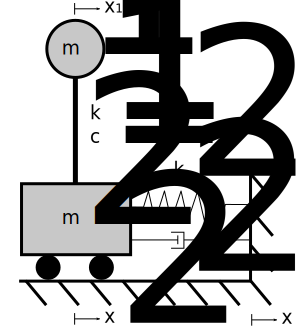
\includegraphics[width=0.5\textwidth]{voigt-kelvin-model.png}
    \caption{Voigt-Kelvin-Modell}
    \label{fig:vkm}
\end{figure}

Unter Annahme der Linearität können die Systeme getrennt betrachtet werden. Am System der Struktur wird durch Parameter Sweeps das Antwortspektrum berechnet. Da der untere Teil des Systems dabei unverändert bleibt kann anschließend durch Komposition das Isolationsspektrum ermittelt werden.
Da das Antwortspektrum für Einmassenschwinger bereits bekannt ist, kann die Betrachtung des Gesamtsystems und eine aufwändige Zeitschrittanalyse entfallen.

\subsection{Bewegungsgleichung}



\pagebreak








\section{Vergleich zum Zweimassenschwinger}
\label{sec:vergleich}

Anahand eines Beispiels soll in einer Handrechnung an einem einfachen System zunächst die auf die aufgehende Struktur wirkende Gesamterdbebenkraft $F_b$ mittels des Isolationsspektrums ermittelt werden und anschließend mit den Ergebnissen einer Berechnung am Zweimassenschwinger verglichen werden.

\begin{figure}[ht]
    \centering
    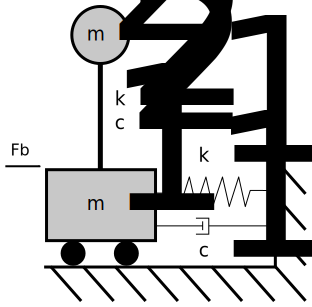
\includegraphics[width=0.5\textwidth]{2MS_beispiel.png}
    \caption{Zweimassenschwinger}
    \label{fig:2ms}
\end{figure}

Die Dämpfung beträgt $c_1 = c_2 = 5\%$, die Masse des Kellergeschosses $m_1 = 0.2 MN/s^2/m$ mit einer Steifigkeit von $k_1 = 5 MN/m$ und die Masse der aufgehenden Struktur $m_2 = 1 MN/s^2/m$ mit einer Steifigkeit von $k_2 = 45 MN/m$.

Das Verhältnis der Eigenkreisfrequenzen der Basis $\omega_1$ zur Struktur $\omega_2$ beträgt somit ungefähr $1/3$. Ein Wert der sich beim Design von Isolatoren in der Praxis bewehrt hat.

\subsection{Bemessungsspektrum}

Für dieses Beispiel wird ein Antwortspektrum aus dem Raum Karlsruhe herangezogen. Damit ergibt sich eine Bodenbeschleunigung in der Erdbebenzone 1 von $a_g = 0.4 m/s^2$ und die Baugrundklasse C-S mit den Kontrollperioden $T_B$, $T_C$, $T_D$ und Untergrundparameter $S$:

\begin{align*}
S &= 0.75 s\\
T_B &= 0.1 s\\
T_C &= 0.5 s\\
T_D &= 2.0 s
\end{align*}

Der Bedeutungsbeiwert wird mit $\gamma_1 = 1.0$ für gewöhnliche Bauten mit Bedeutungsklasse II, der Verstärkungsbeiwert der Spektralbeschleunigung mit $\beta_0 = 2.5$ für eine viskose Dämpfung von 5\% und der Verhaltensbeiwert für Duktilitätsklasse 1 mit $q = 1.5$ angesetzt.
Daraus ergibt sich das Bemessungsspektrum zu \cref{fig:Bemessungsspektrum}.

\begin{figure}[ht] 
    \centering
    \includegraphics[width=0.9\textwidth]{AWS_beispiel.png}
    \caption{Bemessungsspektrum}
    \label{fig:Bemessungsspektrum}
\end{figure}

\subsection{Betrachtung mit Isolationsspektrums}

*Isolationsspektrum zeigen

Die Eigenfrequenz der Struktur ergibt sich zu

\begin{align*}
\omega &= \sqrt{\frac{k_2}{m_2}} = \sqrt{\frac{45}{1}}\\
       &= 6.708 s^{-1}
\end{align*}

\begin{align*}
T &= \frac{2 \cdot \pi}{\omega} = \frac{2 \cdot \pi}{6.708}\\
  &= 0.936 s
\end{align*}

und eine Beschleunigung von

\begin{align*}
S_d(T) &= a_g \cdot \gamma_1 \cdot S \cdot \frac{\beta_0}{q} \cdot \frac{T_C}{T}\\
S_d(0.936) &= 0.4 \cdot 1.0 \cdot 0.75 \cdot \frac{2.5}{1.5} \cdot \frac{0.5}{0.936}\\
           &= 0.277 m/s^2
\end{align*}

Die Übertragungsfunktion für den hier gegebenen Isolator lautet:

\begin{align*}
G(s) &= \frac{1}{m_1 \cdot s^2 + c_1 \cdot s + k_1}\\
     &= \frac{1}{0.2 \cdot s^2 + 0.05 \cdot s + 5}
\end{align*}

Um die Amplitude zu erhalten wird der Laplace-Faktor $s$ bestimmt und der Betrag der Übertragungsfunktion ermittelt.

\begin{align*}
s &= i \cdot \omega\\
  &= i \cdot 6.708\\
  &= 6.708i
\end{align*}

\begin{align*}
|G(6.708i)| &= |\frac{1}{0.2 \cdot 6.708i^2 + 0.05 \cdot 6.708i + 5}|\\
            &= 0.208
\end{align*}

Die an der Struktur wirkende Gesamterdbebenkraft $F_b$ ergibt sich somit zu:

\begin{align*}
F_b &= |G(s)| \cdot S_d(T) \cdot m_2\\
    &= 0.208 \cdot 0.277 m/s^2 \cdot 1 MN/s^2/m\\
    &= \underline{\underline{0.0576 MN}}
\end{align*}

\subsection{Betrachtung am Zweimassenschwinger}

Bei der Betrachtung des Zweimassenschwingers kann vereinfacht angenommen werden, dass der weiche Isolator die Eigentform dominiert \cite{AKK} und sich die Eigenfrequenz des Gesamtsystems somit zu

\begin{align*}
\omega_1 &= \sqrt{\frac{k_1}{m_1 + m_2}}\\
         &= \sqrt{\frac{5}{1.0 + 0.2}}\\
         &= 2.041 s^{-1}
\end{align*}

\begin{align*}
T_1 &= \frac{2 \cdot \pi}{\omega} = \frac{2 \cdot \pi}{2.041}\\
    &= 3.078 s
\end{align*}

ergibt. Die auf die Struktur wirkende Gesamterdbebenkraft $F_b$ ist dann:

\begin{align*}
F_b &= S_d(T) \cdot m_2\\
    &= 0.053 m/s^2 \cdot 1 MN/s^2/m\\
    &= \underline{\underline{0.053 MN}}
\end{align*}

Damit liegt die Abweichung der beiden Ansätze in dem Fall bei $0.0576/0.053=1.0945$, also ungefähr $9.5\%$.

\pagebreak

\section{Grenzfälle}
\label{sec:grenzfalle}

Zur weiteren Untersuchung soll noch eine Berechnung am Zweimassenschwinger mit den Beteiligungsfaktoren der Schwingungsform erfolgen, wobei hier die Steifigkeit des Isolators variiert wird. Die Berechnung mittels Isolationsspektrum erfolgt analog zum vorherigen Beispiel.

Die Eigenkreisfrequenz wird über die Lösung des charakteristischen Polynoms der Matrizenform des Systems der gekoppelten Bewegungsdifferentialgleichungen des Zweimassenschwingers (\cite{Pocanschi} S. 143, Gl. 8.11) ermittelt.

\begin{equation*}
\omega_1 = \sqrt{\frac{(k_1 + k_2) \cdot m_2 + k_2 \cdot m_1 - \sqrt{[(k_1 + k_2) \cdot m_2 + k_2 \cdot  m_1]^2 - 4 \cdot m_1 \cdot m_2 \cdot k_1 \cdot k_2}}{2 \cdot m_1 \cdot m_2}}
\end{equation*}

Und der Beteiligungsfaktor des Isolators zu

\begin{equation*}
X = 1/\left( \frac{k_1 + k_2 - m_1 \cdot \omega_1^2}{k_2} \right)
\end{equation*}

\begin{figure}[ht] 
    \centering
    \includegraphics[width=0.9\textwidth]{DampenerSweep.png}
    \caption{Abweichung der beiden Ansätze}
    \label{fig:Bemessungsspektrum}
\end{figure}

*2MS mit Beteiligungsfaktor  -> Diagramm mit Verschiebung = 1

*Abweichung durch Schwebung/Beteiligung 2. Feder 

\pagebreak

\section{Nichtlinearitäten und Ansätze zur Linearisierung}
\label{sec:nichtlinearitaten}

*Huber

\pagebreak